\documentclass[11pt,a4paper]{article}

% --------------------------------------------------
% PAQUETES
% --------------------------------------------------
\usepackage[utf8]{inputenc}
\usepackage[T1]{fontenc}
\usepackage[spanish,es-nodecimaldot]{babel}
\usepackage{amsmath,amssymb}
\usepackage{graphicx}
\usepackage{booktabs}
\usepackage{array}
\usepackage{float}
\usepackage{geometry}
\usepackage{xcolor}
\usepackage{hyperref}
\usepackage{listings}
\usepackage{caption}
\usepackage{enumitem}
\usepackage[ruled,vlined,linesnumbered]{algorithm2e}
\usepackage{microtype}

\geometry{top=2.5cm,bottom=2.5cm,left=2.5cm,right=2.5cm}

\hypersetup{
    colorlinks=true,
    linkcolor=blue,
    citecolor=blue,
    urlcolor=blue
}

\lstset{
    language=Python,
    basicstyle=\ttfamily\small,
    numbers=left,
    numberstyle=\tiny,
    frame=single,
    breaklines=true,
    showstringspaces=false,
    tabsize=4
}

\SetKwFor{ForPar}{parallel for}{do}{end}
\SetKwComment{tcp}{// }{}

% --------------------------------------------------
% COMANDOS
% --------------------------------------------------
\newcommand{\Tseq}{T_{\mathrm{seq}}}
\newcommand{\Tpar}{T_p}
\newcommand{\Work}{W}
\newcommand{\Depth}{D}
\newcommand{\Speedup}{S}
\newcommand{\Efficiency}{E_f}
\newcommand{\Cost}{C}

\begin{document}

% ==================================================
% PORTADA
% ==================================================
\begin{titlepage}
    \centering
    \vspace*{0.5cm}

    \IfFileExists{UTEC-Logo.jpg}{%
        \includegraphics[width=7.5cm]{UTEC-Logo.jpg}\par\vspace{0.8cm}
    }{}

    {\Large UNIVERSIDAD DE INGENIERÍA Y TECNOLOGÍA\par}
    \vspace{0.5cm}
    {\large Computación Paralela y Distribuida\par}

    \vfill

    {\LARGE\bfseries
    Paralelización PRAM del Entrenamiento de Múltiples\\
    Redes Neuronales MLP\par}

    \vspace{1cm}
    {\large Proyecto Parcial\par}
    {\large Docente: José Fiestas\par}

    \vfill

    \begin{tabular}{lc}
        \toprule
        Integrante & Participación \\
        \midrule
        Noemi Huarino Anchillo   & 100\% \\
        Margiory Alvarado Chavez & 100\% \\
        Mariel Tovar Tolentino   & 100\% \\
        \bottomrule
    \end{tabular}

    \vfill
    Lima, Perú\\
    Septiembre de 2026
\end{titlepage}

\tableofcontents
\newpage

% ==================================================
\section{Introducción}
% ==================================================

El proyecto estudia la paralelización del entrenamiento de múltiples redes neuronales
MLP inicializadas con semillas distintas. El pseudocódigo base evalúa varios modelos
sobre una misma partición de entrenamiento y prueba y selecciona, al finalizar, el
modelo con mayor exactitud. La estructura del algoritmo presenta paralelismo natural:
los entrenamientos correspondientes a semillas diferentes no dependen entre sí y solo
requieren combinar sus resultados al final.

El objetivo es diseñar este procedimiento bajo un modelo PRAM, caracterizar su trabajo,
profundidad, speedup y eficiencia, e implementar una aproximación práctica en Python
para contrastar posteriormente el comportamiento teórico con mediciones experimentales.
El análisis toma como costo base, de acuerdo con el enunciado del proyecto, el
entrenamiento de un MLP:

\begin{equation}
    \Cost(n,d,h,E)=\Theta(E\,n\,d\,h),
    \label{eq:costo-modelo}
\end{equation}

donde $E$ es el número de épocas/iteraciones consideradas por el modelo de costo,
$n$ el número de muestras, $d$ la dimensión de entrada y $h$ el parámetro de ancho
utilizado en la cota proporcionada.

% ==================================================
\section{Formulación del problema y algoritmo secuencial}
% ==================================================

\subsection{Notación}

Para distinguir el tamaño del workload de la cantidad de recursos se emplea la
notación de la Tabla~\ref{tab:notacion}.

\begin{table}[H]
\centering
\begin{tabular}{cl}
\toprule
Símbolo & Descripción \\
\midrule
$E$ & Número de épocas/iteraciones del entrenamiento \\
$n$ & Número de muestras \\
$d$ & Número de características de entrada \\
$h$ & Parámetro de ancho/neuronas usado en la cota del enunciado \\
$m=|S|$ & Número de semillas/modelos evaluados \\
$p$ & Número de procesadores/workers disponibles \\
\bottomrule
\end{tabular}
\caption{Notación empleada en el análisis.}
\label{tab:notacion}
\end{table}

El pseudocódigo del enunciado usa como caso particular
$S=\{0,1,\ldots,p-1\}$, por lo que $m=p$. En el análisis formal se mantienen
$m$ y $p$ separados para no confundir la cantidad de modelos que forman el problema
con el número de recursos asignados. Al final se especializan las expresiones al caso
$m=p$ solicitado.

\subsection{Algoritmo secuencial}

\begin{algorithm}[H]
\caption{Entrenamiento secuencial de múltiples MLP con semillas distintas}
\label{alg:secuencial}
\KwIn{Datos $(X,y)$, conjunto de semillas $S$, hiperparámetros del MLP}
\KwOut{Modelo $M^*$ con mayor exactitud}

Dividir una sola vez $(X,y)$ en train y test\;
$A_{\mathrm{best}}\leftarrow -\infty$; $M^*\leftarrow \varnothing$\;

\ForEach{$s\in S$}{
    Inicializar el generador aleatorio con semilla $s$\;
    Construir el modelo independiente $M_s$\;
    Entrenar $M_s$ sobre el conjunto de entrenamiento\;
    $A_s\leftarrow \operatorname{accuracy}(M_s,X_{\mathrm{test}},y_{\mathrm{test}})$\;
    \If{$A_s>A_{\mathrm{best}}$}{
        $A_{\mathrm{best}}\leftarrow A_s$\;
        $M^*\leftarrow M_s$\;
    }
}
Guardar y retornar $M^*$\;
\end{algorithm}

Si entrenar un modelo cuesta $\Cost=\Theta(E n d h)$, entrenar secuencialmente
$m$ semillas tiene costo

\begin{equation}
    \Tseq(m,n,d,h,E)=\Theta(m\,E\,n\,d\,h).
    \label{eq:tseq-general}
\end{equation}

La comparación final entre las $m$ accuracies añade $\Theta(m)$ operaciones, que no
cambia el orden cuando el costo de entrenamiento domina.

% ==================================================
\section{Diseño del algoritmo PRAM}
% ==================================================

\subsection{Paralelismo entre semillas}

La unidad paralela principal es el entrenamiento completo correspondiente a una semilla.
Para dos semillas distintas $s_i$ y $s_j$, los modelos $M_i$ y $M_j$ poseen estados
mutables independientes: pesos, trayectoria de optimización y resultado final. Por ello,
ambos entrenamientos pueden ejecutarse simultáneamente siempre que compartan únicamente
información de solo lectura, como el dataset, la partición train/test y los hiperparámetros.

Con $m$ semillas y $p$ workers, las semillas se distribuyen entre los workers; cada uno
procesa como máximo $\lceil m/p\rceil$ entrenamientos. En el caso particular $m=p$,
cada worker entrena exactamente un modelo.

\subsection{Elección de CREW-PRAM}

Se adopta el modelo \textbf{CREW (Concurrent Read, Exclusive Write)} porque representa
de manera directa el patrón de acceso requerido:

\begin{itemize}[leftmargin=*]
    \item \textbf{Lecturas concurrentes:} varios procesadores pueden consultar de forma
    simultánea $X_{\mathrm{train}}$, $y_{\mathrm{train}}$, $X_{\mathrm{test}}$,
    $y_{\mathrm{test}}$ y los hiperparámetros comunes.
    \item \textbf{Escrituras exclusivas:} cada semilla escribe su accuracy y la referencia
    a su modelo en posiciones propias, por ejemplo $Acc[s]$ y $Mod[s]$.
\end{itemize}

No se requiere CRCW porque el algoritmo evita que dos procesadores escriban
simultáneamente en la misma celda. Un diseño EREW también sería posible mediante
replicación o planificación adicional de lecturas; sin embargo, CREW se ajusta de forma
más natural a la lectura compartida del dataset sin introducir esa complejidad extra.

\subsection{Pseudocódigo paralelo teórico}

\begin{algorithm}[H]
\caption{Entrenamiento paralelo CREW-PRAM de múltiples MLP}
\label{alg:crew}
\KwIn{Datos $(X,y)$, semillas $S$ con $|S|=m$, $p$ procesadores}
\KwOut{Modelo $M^*$ con mayor exactitud}

$P_0$ divide una sola vez los datos en train/test y publica los datos de solo lectura\;

\ForPar{$P_i$, $i=0,\ldots,p-1$}{
    \For{$s=i$; $s<m$; $s\leftarrow s+p$}{
        Construir y entrenar $M_s$ con semilla $s$\;
        $Acc[s]\leftarrow \operatorname{accuracy}(M_s)$\;
        $Mod[s]\leftarrow M_s$\;
        \tcp{cada $s$ tiene un slot exclusivo}
    }
}

Realizar reducción binaria sobre $(Acc[s],Mod[s])$ para obtener el máximo global\;
$P_0$ guarda y retorna el modelo ganador\;
\end{algorithm}

La reducción se organiza como un árbol binario. En cada nivel se comparan pares
disjuntos, por lo que ninguna posición destino recibe dos escrituras simultáneas. La
profundidad de esta fase es $\Theta(\log m)$.

% ==================================================
\section{Análisis de complejidad PRAM}
% ==================================================

\subsection{Trabajo}

El trabajo total incluye $m$ entrenamientos de costo $\Cost$ y una reducción de máximo
con $m-1$ comparaciones:

\begin{align}
    \Work
    &= \Theta(m\Cost+m) \\
    &= \Theta(m\,E\,n\,d\,h).
    \label{eq:work}
\end{align}

Este orden coincide con el algoritmo secuencial para el mismo conjunto de $m$ semillas,
por lo que la estrategia es work-optimal respecto de este baseline.

\subsection{Profundidad}

En esta versión del diseño el paralelismo se explota \emph{entre} modelos; el
entrenamiento interno de cada MLP se considera una cadena de costo $\Cost$. Con
procesadores suficientes, todos los entrenamientos pueden ejecutarse simultáneamente y,
después, la reducción requiere $\Theta(\log m)$ niveles:

\begin{equation}
    \Depth=\Theta(\Cost+\log m)
    =\Theta(E\,n\,d\,h+\log m).
    \label{eq:depth}
\end{equation}

\subsection{Paralelismo disponible}

\begin{equation}
    \Pi=\frac{\Work}{\Depth}
    =\Theta\left(\frac{m\Cost}{\Cost+\log m}\right).
    \label{eq:parallelism}
\end{equation}

Cuando $\Cost\gg\log m$, se obtiene $\Pi\approx\Theta(m)$. Por tanto, el número de
semillas limita esencialmente el paralelismo externo aprovechable: disponer de muchos
más procesadores que modelos no reduce el costo secuencial interno de un entrenamiento.

\subsection{Tiempo con $p$ procesadores}

Distribuyendo $m$ semillas entre $p$ workers, un modelo de tiempo directo es

\begin{equation}
    \Tpar(m,p)=\Theta\left(\left\lceil\frac{m}{p}\right\rceil\Cost+\log m\right).
    \label{eq:tp-directo}
\end{equation}

La Ley de Brent proporciona además la cota general

\begin{equation}
    \Tpar=O\left(\frac{\Work}{p}+\Depth\right)
    =O\left(\frac{m\Cost}{p}+\Cost+\log m\right).
    \label{eq:brent}
\end{equation}

\subsection{Caso particular $m=p$}

El enunciado define $S=\{0,1,\ldots,p-1\}$, de modo que $m=p$. En esta configuración,
el workload contiene $p$ entrenamientos y cada worker procesa uno:

\begin{equation}
    T_{\mathrm{par}}(p)=\Theta(\Cost+\log p).
    \label{eq:tpar-mp}
\end{equation}

El mismo workload ejecutado secuencialmente requiere

\begin{equation}
    T_{\mathrm{seq}}(p)=\Theta(p\Cost).
    \label{eq:tseq-mp}
\end{equation}

Por tanto, el speedup teórico para \emph{el mismo conjunto de $p$ semillas} es

\begin{equation}
    \Speedup(p)
    \approx\frac{p\Cost}{\Cost+\log p},
    \label{eq:speedup}
\end{equation}

y la eficiencia es

\begin{equation}
    \Efficiency(p)=\frac{\Speedup(p)}{p}
    \approx\frac{\Cost}{\Cost+\log p}.
    \label{eq:eficiencia}
\end{equation}

Si $\Cost\gg\log p$, entonces $\Speedup(p)\approx p$ y $\Efficiency(p)\approx1$ en el
modelo ideal. Estas expresiones no incluyen creación de procesos, serialización, copias
de memoria, scheduling ni paralelismo interno de las bibliotecas numéricas.

\subsection{Criterio correcto para medir speedup}

Debido a que el caso $m=p$ aumenta el número de modelos cuando aumenta $p$, no es
correcto usar el tiempo de $p=1$ como baseline secuencial para todos los puntos. Para
cada valor de $p$ se debe comparar el mismo workload:

\begin{equation}
    \Speedup(p)=
    \frac{T_{\mathrm{seq}}(m=p)}{T_{\mathrm{par}}(m=p,p)}.
    \label{eq:speedup-experimental}
\end{equation}

Es decir, el baseline secuencial correspondiente a $p=8$ debe entrenar las mismas ocho
semillas una tras otra antes de compararse con la ejecución paralela de esas ocho
semillas.

% ==================================================
\section{Implementación y estado de las versiones beta}
% ==================================================

\subsection{Tecnologías y mapeo del modelo}

La implementación actual se desarrolla en Python con \texttt{scikit-learn}. La Beta 1
utiliza \texttt{MLPClassifier} para los modelos, \texttt{make\_classification} para
generar datasets sintéticos de tamaño controlado, \texttt{train\_test\_split} para una
partición reproducible y \texttt{multiprocessing.Pool} para ejecutar entrenamientos de
semillas distintas en procesos separados.

La elección de procesos, en lugar de \texttt{threading}, busca obtener paralelismo CPU
real para un workload computacional. En el modelo teórico, $p$ representa procesadores
PRAM; en la Beta 1, $p$ se mapea a procesos worker del sistema operativo.

\paragraph{Limitación importante.}
CREW presupone una memoria global compartida. En la implementación actual, los arreglos
de NumPy se pasan como argumentos a los workers. En plataformas que usan
\emph{spawn}, como Windows, esto implica serialización y copias; por ello la Beta 1 es
una aproximación del patrón de tareas CREW, no una realización literal de su memoria
compartida. Esta diferencia deberá considerarse al analizar el overhead experimental.

\subsection{Beta 0: baseline secuencial}

La Beta 0 implementa el baseline secuencial del algoritmo. Su función es entrenar
exactamente el mismo conjunto de $m$ semillas que la versión paralela, pero una tras
otra. Esta condición es necesaria para que la comparación de tiempos utilice el mismo
workload y para que el speedup no mezcle una reducción del tiempo con una reducción de
la cantidad de modelos entrenados.

La implementación se encuentra en\linebreak
\texttt{src/beta0\_sequential.py}. La partición de los datos se realiza una sola vez
antes del bucle de semillas, utilizando el mismo tamaño de prueba y la misma semilla de
partición que Beta 1. Para cada $s\in\{0,\ldots,m-1\}$, el programa construye un
\texttt{MLPClassifier} con \texttt{random\_state=s}, entrena el modelo, calcula su
accuracy y actualiza el ganador si obtiene un valor mayor.

En el experimento definido por el enunciado se utiliza $m=p$. Por tanto, para medir el
speedup correspondiente a un valor de $p$, la Beta 0 entrena secuencialmente las mismas
$p$ semillas que la Beta 1 ejecuta con $p$ workers. La medición se realiza alrededor del
entrenamiento completo, incluyendo la división de datos, el entrenamiento de todas las
semillas y la selección del mejor resultado.

La estructura principal de la Beta 0 es:

\begin{lstlisting}
X_train, X_test, y_train, y_test = train_test_split(
    X, y, test_size=test_size, random_state=split_seed
)

for seed in range(m):
    modelo = MLPClassifier(random_state=seed, ...)
    modelo.fit(X_train, y_train)
    accuracy = accuracy_score(y_test, modelo.predict(X_test))

    if accuracy > mejor_accuracy:
        mejor_accuracy = accuracy
        mejor_seed = seed
        mejor_modelo = modelo
\end{lstlisting}

El programa también registra el tiempo individual de cada semilla, además del tiempo
total del baseline. Esta información permite detectar anomalías, como una semilla cuyo
entrenamiento tarde considerablemente más que las demás. La reproducibilidad se controla
manteniendo fijos el dataset, la partición train/test, los hiperparámetros y la semilla
aleatoria de cada modelo.

\subsection{Beta 1: paralelismo entre semillas}

La Beta 1 implementada ejecuta una tarea por semilla mediante
\texttt{multiprocessing.Pool}. Cada worker construye un modelo independiente, calcula
su accuracy y devuelve $(seed,accuracy,modelo)$ al proceso maestro. La estructura
principal puede resumirse como:

\begin{lstlisting}
with Pool(processes=p) as pool:
    resultados = pool.map(_entrenar_una_semilla, tareas)

mejor_seed, mejor_acc, mejor_modelo = max(
    resultados, key=lambda r: r[1]
)
\end{lstlisting}

La paralelización de los entrenamientos coincide con el diseño PRAM. Sin embargo, la
selección actual del máximo se realiza secuencialmente mediante \texttt{max}, con costo
$\Theta(m)$ en el maestro. La reducción en árbol $\Theta(\log m)$ pertenece al diseño
teórico y debe incorporarse en una beta posterior si se busca una correspondencia más
estrecha entre código y pseudocódigo PRAM.

La configuración actual de Beta 1 es provisional. El código utiliza por defecto
\texttt{hidden\_layer\_sizes=(10,10)}, $\alpha=10^{-4}$,
\texttt{learning\_rate\_init}$=10^{-3}$ y \texttt{max\_iter}$=200$. El informe mantiene
$\Theta(E n d h)$ como el modelo de costo indicado por el enunciado; antes de la campaña
experimental final, el equipo debe congelar la arquitectura e hiperparámetros y no
modificarlos entre configuraciones.

\subsubsection{Validación de la semántica paralela}

Para comprobar que la paralelización conserva la lógica del algoritmo secuencial, se
compararon Beta 0 y Beta 1 utilizando el mismo dataset, la misma partición train/test,
los mismos hiperparámetros y las mismas semillas para cada valor de $p$. Las pruebas se
realizaron con $n=5000$ muestras y $p\in\{1,2,4\}$. En cada caso se utilizó
$m=p$, por lo que ambas versiones procesaron el mismo workload.

\begin{table}[H]
\centering
\begin{tabular}{c r r c c c c}
\toprule
$p=m$ & $T_{\mathrm{seq}}$ (s) & $T_{\mathrm{par}}$ (s) &
Semilla sec. & Semilla par. & Acc. sec. & Acc. par. \\
\midrule
1 & 2.4544 & 5.5927 & 0 & 0 & 0.9630 & 0.9630 \\
2 & 5.5678 & 6.0055 & 1 & 1 & 0.9700 & 0.9700 \\
4 & 10.0961 & 6.3861 & 1 & 1 & 0.9700 & 0.9700 \\
\bottomrule
\end{tabular}
\caption{Validación inicial de Beta 0 y Beta 1 con $n=5000$.}
\label{tab:validacion-beta}
\end{table}

En los tres casos, Beta 0 y Beta 1 seleccionaron la misma mejor semilla y obtuvieron la
misma accuracy. Para $p=1$ la mejor semilla fue $0$, mientras que para $p=2$ y $p=4$
fue $1$. Esto indica que la ejecución paralela conserva la lógica funcional de Beta 0:
cada semilla entrena un modelo independiente y la selección final se realiza sobre el
mismo conjunto de resultados.

El speedup y la eficiencia se calcularon comparando el mismo workload secuencial y
paralelo para cada valor de $p$:

\begin{table}[H]
\centering
\begin{tabular}{c c c}
\toprule
$p$ & Speedup $S(p)$ & Eficiencia $E_f(p)$ \\
\midrule
1 & $0.4388$ & $43.88\%$ \\
2 & $0.9271$ & $46.36\%$ \\
4 & $1.5809$ & $39.52\%$ \\
\bottomrule
\end{tabular}
\caption{Speedup y eficiencia de la validación inicial.}
\label{tab:metricas-validacion}
\end{table}

Por ejemplo, para $p=4$:

\begin{equation}
    S(4)=\frac{T_{\mathrm{seq}}(4)}{T_{\mathrm{par}}(4)}
    =\frac{10.0961}{6.3861}\approx 1.5809,
    \qquad
    E_f(4)=\frac{1.5809}{4}\approx 39.52\%.
\end{equation}

Estos valores corresponden a una validación inicial, no al benchmark final. La
diferencia respecto al speedup ideal se atribuye preliminarmente a la creación de
procesos, la transferencia o copia de datos y la reducción secuencial realizada por el
proceso maestro. En particular, para $p=1$ y $p=2$ el costo adicional de crear procesos
supera el beneficio de la ejecución concurrente. A partir de $p=4$, el costo de los
entrenamientos comienza a compensar parcialmente dicho overhead.

\subsection{Benchmark Beta 1}

El script \texttt{benchmarks/run\_benchmarkB1.py} automatiza combinaciones de

\begin{equation}
    p\in\{1,2,4,8,16,32\},\qquad
    n\in\{5000,10000,20000,40000\},
\end{equation}

realiza varias repeticiones y registra tiempo promedio, mínimo, máximo y accuracy. Esta
fase permite estudiar el costo real de la Beta 1, pero todavía no constituye el benchmark
final de speedup mientras no se incluya el baseline secuencial equivalente para cada
workload.

% ==================================================
\section{Metodología experimental}
% ==================================================

La campaña final deberá mantener constantes arquitectura, hiperparámetros, número de
features, proporción train/test, seed de generación del dataset, seed del split y entorno
de ejecución. Para cada combinación se recomienda realizar al menos tres repeticiones y
reportar tanto una medida central como la dispersión observada.

El dataset sintético es apropiado para este objetivo porque permite fijar exactamente el
número de muestras sin introducir cambios de distribución entre valores de $p$. La Beta
1 actual genera datos binarios con \texttt{n\_features=20},
\texttt{n\_informative=15} y \texttt{random\_state=42}.

\subsection{Control del paralelismo interno}

Las bibliotecas numéricas utilizadas por scikit-learn pueden ejecutar operaciones BLAS
con múltiples hilos. Si cada proceso worker crea a su vez varios hilos internos se produce
\emph{oversubscription}; en tal caso, $p$ deja de representar adecuadamente el número de
recursos externos estudiado. Antes de medir resultados finales se deben limitar y
documentar los hilos internos de OpenMP/BLAS, por ejemplo mediante variables de entorno
o \texttt{threadpoolctl}.

\subsection{Métricas}

Para cada configuración se registrarán al menos:

\begin{align}
    T_{\mathrm{seq}}(p,n),\qquad
    T_{\mathrm{par}}(p,n),\qquad
    \Speedup(p,n)&=\frac{T_{\mathrm{seq}}(p,n)}{T_{\mathrm{par}}(p,n)},\\
    \Efficiency(p,n)&=\frac{\Speedup(p,n)}{p}.
\end{align}

% ==================================================
\section{Resultados y comparación teoría--experimento}
% ==================================================

% TODO MARGIORY: insertar resultados finales y figuras una vez terminados los benchmarks.
A la fecha de este avance se dispone de la infraestructura inicial para medir tiempos de
Beta 1. La comparación final deberá superponer el comportamiento experimental con el
modelo teórico, considerando que la constante multiplicativa de la notación asintótica
se estima a partir de mediciones y se mantiene fija al generar predicciones posteriores.

Si $\Cost=c\,E n d h$ para una constante empírica $c$, el caso $m=p$ predice

\begin{equation}
    T_{\mathrm{par,teo}}(p,n)
    \approx c\,E n d h + c_r\log p,
\end{equation}

donde $c_r$ captura el costo de una etapa de reducción en el modelo ajustado. La Beta 1
real puede apartarse de esta forma por serialización, creación de procesos, copias de
datos y reducción secuencial.

\IfFileExists{figures/tiempo.png}{
\begin{figure}[H]
    \centering
    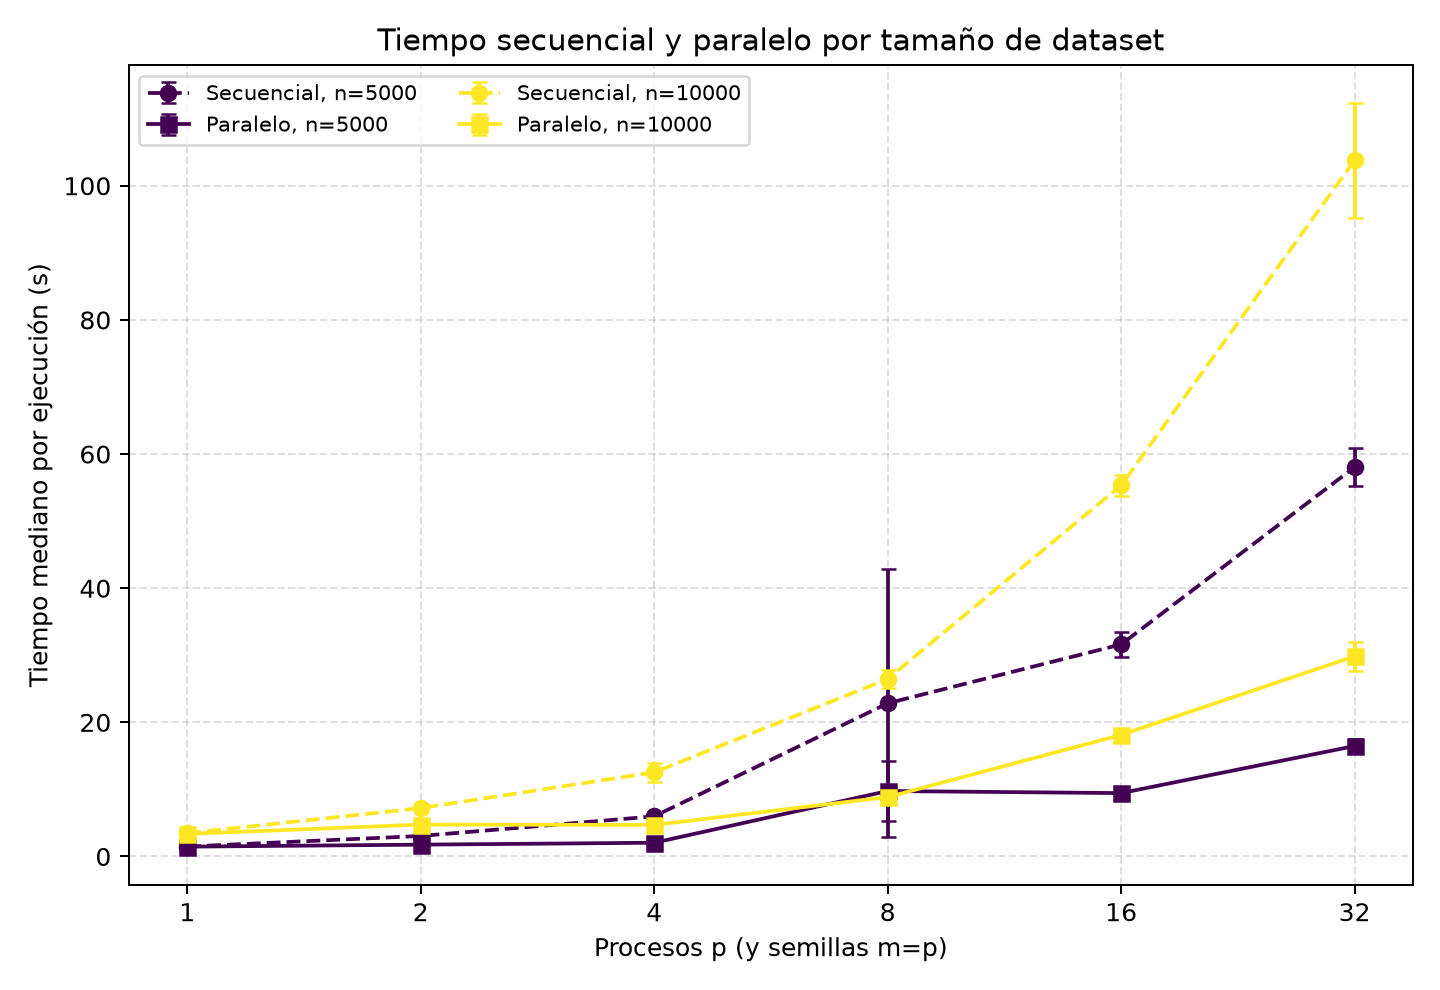
\includegraphics[width=0.8\textwidth]{figures/tiempo.png}
    \caption{Tiempo de ejecución en función del número de workers.}
\end{figure}
}{}

\IfFileExists{figures/speedup.png}{
\begin{figure}[H]
    \centering
    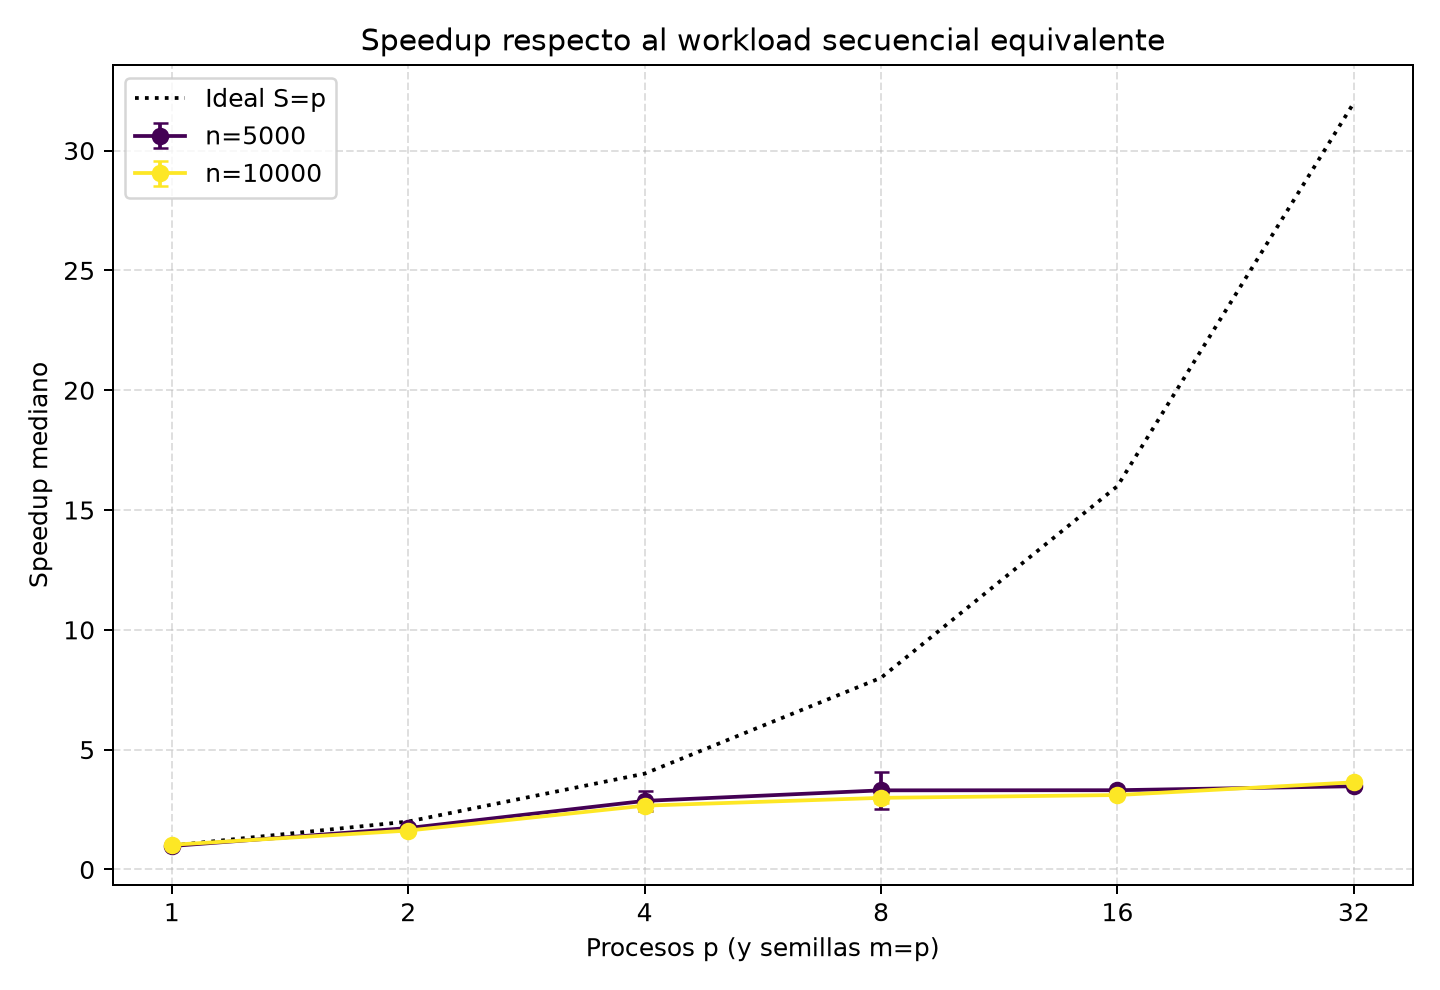
\includegraphics[width=0.8\textwidth]{figures/speedup.png}
    \caption{Speedup experimental.}
\end{figure}
}{}

\IfFileExists{figures/eficiencia.png}{
\begin{figure}[H]
    \centering
    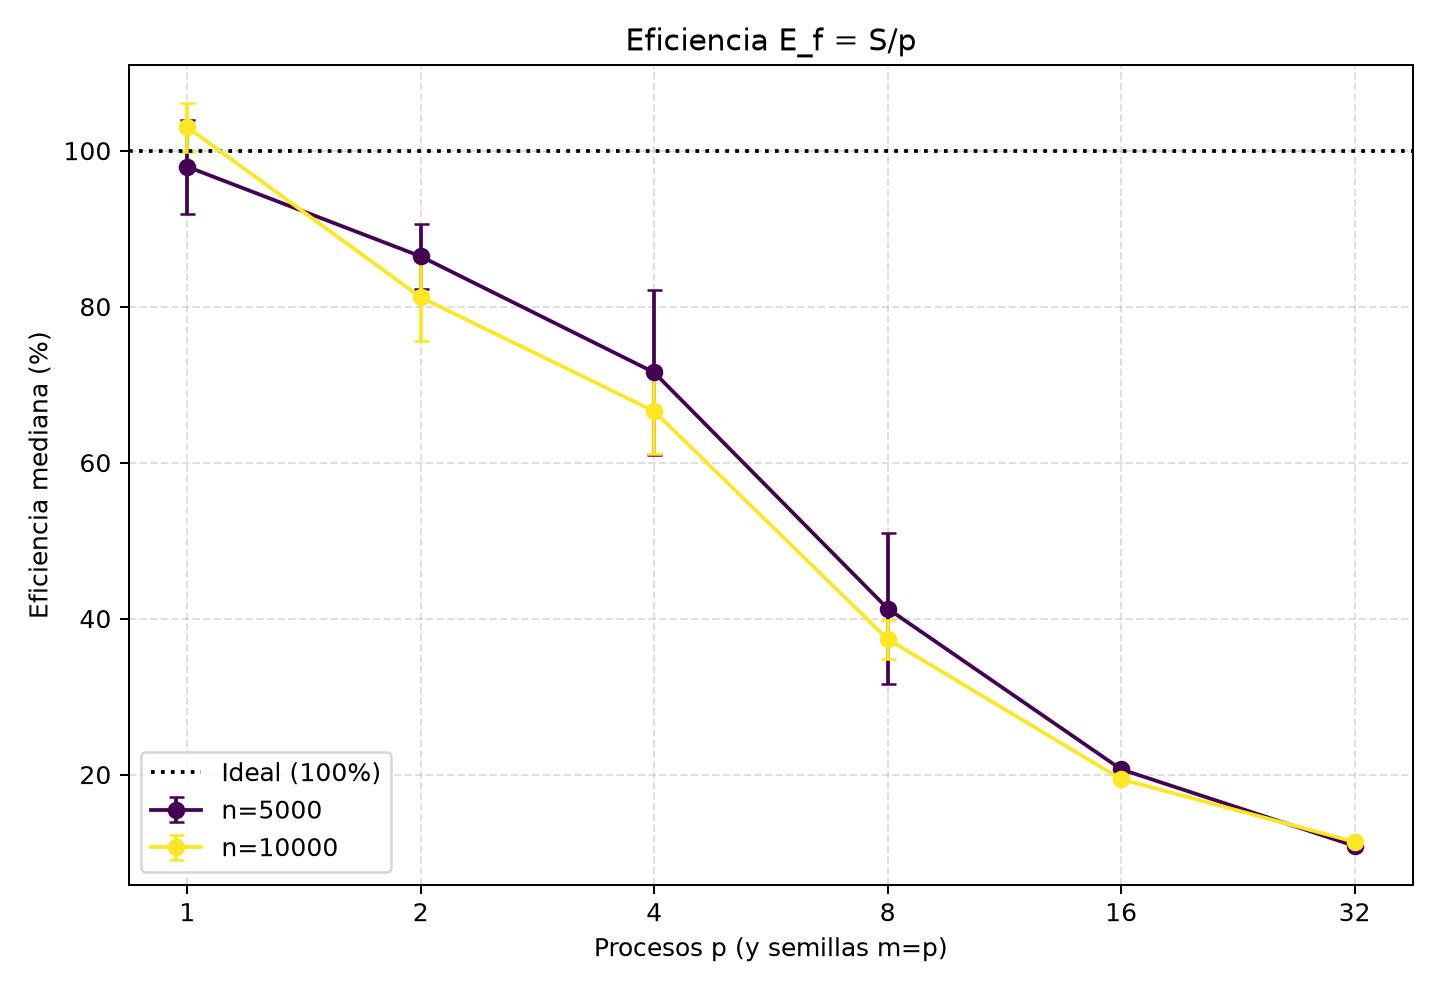
\includegraphics[width=0.8\textwidth]{figures/eficiencia.png}
    \caption{Eficiencia experimental.}
\end{figure}
}{}

% ==================================================
\section{Análisis de escalabilidad}
% ==================================================

% TODO MARGIORY/MARIEL: completar con los resultados finales.
La estrategia externa posee, idealmente, paralelismo máximo del orden de $m$, porque
cada semilla proporciona una tarea independiente. Por ello, incluso bajo PRAM, aumentar
$p$ más allá del número de semillas no reduce el costo interno de un MLP. En la
implementación real también se espera que el overhead de creación de procesos,
movimiento de datos y sincronización reduzca la eficiencia antes de alcanzar el límite
ideal.

Cuando el experimento usa $m=p$, cada punto incrementa simultáneamente la cantidad de
trabajo (más semillas) y los recursos. Por tanto, este conjunto de puntos no debe
interpretarse como strong scaling clásico de un workload fijo. El análisis de speedup se
realiza comparando, para cada $p$, las versiones secuencial y paralela del mismo conjunto
de $p$ semillas.

% ==================================================
\section{Impacto de las fuentes utilizadas}
% ==================================================

Las fuentes se utilizaron para respaldar decisiones concretas del diseño, y no solamente
para incluir definiciones generales. El material oficial del curso fija el problema, el
costo base $\Theta(E n d h)$, los tamaños de $p$ y $n$ y el pseudocódigo de referencia
\cite{fiestas2026proyecto}. Por ello, el repositorio conserva esa expresión como baseline
y no reemplaza el análisis por una cota genérica de multiplicación de matrices.

El libro de Grama, Gupta, Karypis y Kumar se utilizó para organizar el análisis en
trabajo, profundidad, paralelismo, tiempo con $p$ procesadores, speedup y eficiencia
\cite{grama2003}. Esta referencia influyó en la separación entre el trabajo total de las
$m$ semillas y la profundidad del entrenamiento de una semilla más la reducción final.

La documentación oficial de Python sobre \texttt{multiprocessing} respaldó la elección
de procesos para la Beta 1. Esta biblioteca permite ejecutar tareas en procesos
separados y aprovechar varios procesadores, pero también hizo necesario documentar el
costo de creación de procesos y la serialización de datos en Windows
\cite{pythonmultiprocessing}. Por ello, la implementación se presenta como una
aproximación práctica del patrón CREW, no como memoria compartida PRAM literal.

La documentación oficial de scikit-learn se utilizó para verificar el comportamiento de
\texttt{MLPClassifier}, sus parámetros, la inicialización mediante \texttt{random\_state}
y el entrenamiento del clasificador MLP \cite{sklearnmlp}. Esta fuente también evita
afirmar que la implementación actual usa SGD explícitamente: mientras el código no
establezca otro solver, se debe reportar la configuración real de \texttt{MLPClassifier}.

Finalmente, el libro de Goodfellow, Bengio y Courville se utiliza como referencia
conceptual para la red MLP, la propagación hacia adelante, la retropropagación y la
optimización de redes neuronales \cite{goodfellow2016}. Su impacto se limita a la
interpretación del núcleo de entrenamiento; los costos concretos del proyecto se toman
del enunciado oficial del curso.

% ==================================================
\section{Uso de herramientas de inteligencia artificial}
% ==================================================

Se utilizó ChatGPT como herramienta de apoyo durante el desarrollo del proyecto. Las
consultas se enfocaron en organizar el análisis CREW-PRAM, revisar la correspondencia
entre el pseudocódigo y la implementación, derivar speedup y eficiencia, y mejorar la
redacción del informe.

La IA no se utilizó como sustituto de las mediciones ni como fuente experimental. El
equipo verificó manualmente las propuestas contra el enunciado del curso, el código del
repositorio y la documentación oficial de Python y scikit-learn. También se corrigieron
las recomendaciones que no coincidían con la implementación actual, como distinguir el
paralelismo entre semillas del paralelismo interno de las operaciones matriciales y
separar el modelo teórico CREW del costo real de \texttt{multiprocessing}.

% ==================================================
\section{Conclusiones preliminares}
% ==================================================

El pseudocódigo del proyecto permite explotar un nivel de paralelismo de grano grueso
entre semillas: cada entrenamiento es independiente y solo existe una dependencia global
al seleccionar el mejor modelo. Bajo este diseño, CREW es un modelo apropiado porque
permite lectura concurrente del dataset y escrituras exclusivas de los estados y
resultados de cada modelo.

El análisis distingue explícitamente $m$, número de semillas, de $p$, número de recursos.
Esta separación permite formular correctamente el trabajo
$\Theta(m E n d h)$, la profundidad $\Theta(E n d h+\log m)$ y el límite de paralelismo,
que es aproximadamente $\Theta(m)$ cuando el entrenamiento domina el costo de la
reducción.

La Beta 1 ya implementa el paralelismo entre semillas, pero conserva dos diferencias
respecto del PRAM ideal: los datos no se encuentran todavía en memoria compartida literal
y la selección del máximo se realiza secuencialmente en el maestro. Estas diferencias se
considerarán explícitamente al interpretar los benchmarks y constituyen los principales
puntos de mejora para las siguientes versiones.

% ==================================================
\section*{Referencias}
% ==================================================

\bibliographystyle{plain}
\bibliography{references}

\end{document}